\documentclass{standalone}

% Plotting
\usepackage{tikz}
\usetikzlibrary{decorations.markings}
\usetikzlibrary{calc}
% quantikz breaks tikz-cd, see https://tex.stackexchange.com/questions/618330/quantikz-breaks-spacing-in-tikz-matrices-tikz-cd
%\usetikzlibrary{quantikz}
\usetikzlibrary{cd}
\usepackage{pgfplots}

\usepackage{simpler-wick}
\usepackage{physics}

\usepackage{amsmath}
\usepackage{mathtools}

\begin{document}
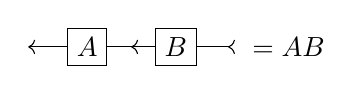
\begin{tikzpicture}[xscale=1.5]
    \draw (0, 0) node[rectangle, draw] (a) {$A$};
    \draw[->] (a) -- ++(-0.5, 0);
    \draw (0.75, 0) node[rectangle, draw] (b) {$B$};
    \draw[-<] (b) -- ++(0.5, 0) node (bin){};
    
    \draw (bin) node[anchor=west] {${}= AB$};
    \begin{scope}[,decoration={
        markings,
        mark=at position 0.5 with {\arrow{>}}}]
        \draw[postaction={decorate}] (b) -- (a);
    \end{scope}
\end{tikzpicture}
\end{document}